% Figure from MATH 493 notes, section 50 (lecture 10/30, Jordan-Hoelder).
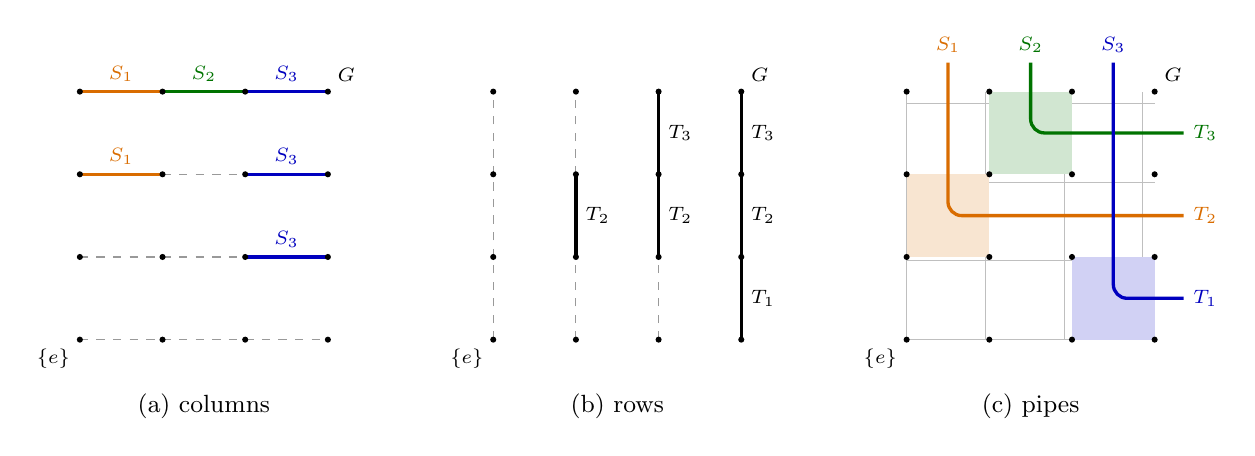
\begin{tikzpicture}[x=1.05cm, y=1.05cm]
\begin{scope}
\draw[black!40, dashed] (0,0) -- (1,0);
\draw[black!40, dashed] (0,1) -- (1,1);
\draw[orange!85!black, very thick] (0,2) -- (1,2); \node[above, orange!85!black, font=\scriptsize] at (0.5,2) {$S_1$};
\draw[orange!85!black, very thick] (0,3) -- (1,3); \node[above, orange!85!black, font=\scriptsize] at (0.5,3) {$S_1$};
\draw[black!40, dashed] (1,0) -- (2,0);
\draw[black!40, dashed] (1,1) -- (2,1);
\draw[black!40, dashed] (1,2) -- (2,2);
\draw[green!45!black, very thick] (1,3) -- (2,3); \node[above, green!45!black, font=\scriptsize] at (1.5,3) {$S_2$};
\draw[black!40, dashed] (2,0) -- (3,0);
\draw[blue!75!black, very thick] (2,1) -- (3,1); \node[above, blue!75!black, font=\scriptsize] at (2.5,1) {$S_3$};
\draw[blue!75!black, very thick] (2,2) -- (3,2); \node[above, blue!75!black, font=\scriptsize] at (2.5,2) {$S_3$};
\draw[blue!75!black, very thick] (2,3) -- (3,3); \node[above, blue!75!black, font=\scriptsize] at (2.5,3) {$S_3$};
\foreach \i in {0,...,3} \foreach \j in {0,...,3} \fill (\i,\j) circle (1.1pt);
\node[below left, font=\scriptsize] at (0,0) {$\{e\}$}; \node[above right, font=\scriptsize] at (3,3) {$G$};
\node[font=\small] at (1.5,-0.8) {(a) columns};
\end{scope}
\begin{scope}[shift={(5.0,0)}]
\draw[black!40, dashed] (0,0) -- (0,1);
\draw[black!40, dashed] (1,0) -- (1,1);
\draw[black!40, dashed] (2,0) -- (2,1);
\draw[black, very thick] (3,0) -- (3,1); \node[right, font=\scriptsize] at (3,0.5) {$T_1$};
\draw[black!40, dashed] (0,1) -- (0,2);
\draw[black, very thick] (1,1) -- (1,2); \node[right, font=\scriptsize] at (1,1.5) {$T_2$};
\draw[black, very thick] (2,1) -- (2,2); \node[right, font=\scriptsize] at (2,1.5) {$T_2$};
\draw[black, very thick] (3,1) -- (3,2); \node[right, font=\scriptsize] at (3,1.5) {$T_2$};
\draw[black!40, dashed] (0,2) -- (0,3);
\draw[black!40, dashed] (1,2) -- (1,3);
\draw[black, very thick] (2,2) -- (2,3); \node[right, font=\scriptsize] at (2,2.5) {$T_3$};
\draw[black, very thick] (3,2) -- (3,3); \node[right, font=\scriptsize] at (3,2.5) {$T_3$};
\foreach \i in {0,...,3} \foreach \j in {0,...,3} \fill (\i,\j) circle (1.1pt);
\node[below left, font=\scriptsize] at (0,0) {$\{e\}$}; \node[above right, font=\scriptsize] at (3,3) {$G$};
\node[font=\small] at (1.5,-0.8) {(b) rows};
\end{scope}
\begin{scope}[shift={(10.0,0)}]
\draw[black!25] (0,0) grid (3,3);
\fill[orange!85!black!18] (0,1) rectangle (1,2);
\fill[green!45!black!18] (1,2) rectangle (2,3);
\fill[blue!75!black!18] (2,0) rectangle (3,1);
\draw[orange!85!black, very thick, rounded corners=5pt] (0.5,3.35) -- (0.5,1.5) -- (3.35,1.5);
\node[above, orange!85!black, font=\scriptsize] at (0.5,3.35) {$S_1$};
\node[right, orange!85!black, font=\scriptsize] at (3.35,1.5) {$T_2$};
\draw[green!45!black, very thick, rounded corners=5pt] (1.5,3.35) -- (1.5,2.5) -- (3.35,2.5);
\node[above, green!45!black, font=\scriptsize] at (1.5,3.35) {$S_2$};
\node[right, green!45!black, font=\scriptsize] at (3.35,2.5) {$T_3$};
\draw[blue!75!black, very thick, rounded corners=5pt] (2.5,3.35) -- (2.5,0.5) -- (3.35,0.5);
\node[above, blue!75!black, font=\scriptsize] at (2.5,3.35) {$S_3$};
\node[right, blue!75!black, font=\scriptsize] at (3.35,0.5) {$T_1$};
\foreach \i in {0,...,3} \foreach \j in {0,...,3} \fill (\i,\j) circle (1.1pt);
\node[below left, font=\scriptsize] at (0,0) {$\{e\}$}; \node[above right, font=\scriptsize] at (3,3) {$G$};
\node[font=\small] at (1.5,-0.8) {(c) pipes};
\end{scope}
\end{tikzpicture}
